

\documentclass[12pt]{article}
\usepackage{amsmath}
\usepackage{latexsym}
\usepackage{amsfonts}
\usepackage[normalem]{ulem}
\usepackage{array}
\usepackage{amssymb}
\usepackage{graphicx}
\usepackage[backend=biber,
style=numeric,
sorting=none,
isbn=false,
doi=false,
url=false,
]{biblatex}\addbibresource{bibliography.bib}

\usepackage{subfig}
\usepackage{wrapfig}
\usepackage{wasysym}
\usepackage{enumitem}
\usepackage{adjustbox}
\usepackage{ragged2e}
|\usepackage[svgnames,table]{xcolor}
\usepackage{tikz}
\usepackage{longtable}
\usepackage{changepage}
\usepackage{setspace}
\usepackage{hhline}
\usepackage{multicol}
\usepackage{tabto}
\usepackage{float}
\usepackage{multirow}
\usepackage{makecell}
\usepackage{fancyhdr}
\usepackage[toc,page]{appendix}
\usepackage[hidelinks]{hyperref}
\usetikzlibrary{shapes.symbols,shapes.geometric,shadows,arrows.meta}
\tikzset{>={Latex[width=1.5mm,length=2mm]}}
\usepackage{flowchart}\usepackage[paperheight=11.0in,paperwidth=8.5in,left=0.5in,right=0.5in,top=0.5in,bottom=0.5in,headheight=1in]{geometry}
\usepackage[utf8]{inputenc}
\usepackage[T1]{fontenc}
\TabPositions{0.49in,0.98in,1.47in,1.96in,2.45in,2.94in,3.43in,3.92in,4.41in,4.9in,5.39in,5.88in,6.37in,6.86in,7.35in,}

\urlstyle{same}


 %%%%%%%%%%%%  Set Depths for Sections  %%%%%%%%%%%%%%

% 1) Section
% 1.1) SubSection
% 1.1.1) SubSubSection
% 1.1.1.1) Paragraph
% 1.1.1.1.1) Subparagraph


\setcounter{tocdepth}{5}
\setcounter{secnumdepth}{5}


 %%%%%%%%%%%%  Set Depths for Nested Lists created by \begin{enumerate}  %%%%%%%%%%%%%%


\setlistdepth{9}
\renewlist{enumerate}{enumerate}{9}
		\setlist[enumerate,1]{label=\arabic*)}
		\setlist[enumerate,2]{label=\alph*)}
		\setlist[enumerate,3]{label=(\roman*)}
		\setlist[enumerate,4]{label=(\arabic*)}
		\setlist[enumerate,5]{label=(\Alph*)}
		\setlist[enumerate,6]{label=(\Roman*)}
		\setlist[enumerate,7]{label=\arabic*}
		\setlist[enumerate,8]{label=\alph*}
		\setlist[enumerate,9]{label=\roman*}

\renewlist{itemize}{itemize}{9}
		\setlist[itemize]{label=$\cdot$}
		\setlist[itemize,1]{label=\textbullet}
		\setlist[itemize,2]{label=$\circ$}
		\setlist[itemize,3]{label=$\ast$}
		\setlist[itemize,4]{label=$\dagger$}
		\setlist[itemize,5]{label=$\triangleright$}
		\setlist[itemize,6]{label=$\bigstar$}
		\setlist[itemize,7]{label=$\blacklozenge$}
		\setlist[itemize,8]{label=$\prime$}

\setlength{\topsep}{0pt}\setlength{\parskip}{8.04pt}
\setlength{\parindent}{0pt}

 %%%%%%%%%%%%  This sets linespacing (verticle gap between Lines) Default=1 %%%%%%%%%%%%%%


\renewcommand{\arraystretch}{1.3}


%%%%%%%%%%%%%%%%%%%% Document code starts here %%%%%%%%%%%%%%%%%%%%



\begin{document}
\begin{Center}
\textbf{EV 2\_8 CALCULAR LOS PARÁMETROS DE ACTIVACIÓN DE TRANSISTORES DE POTENCIA}
\end{Center}\par



%%%%%%%%%%%%%%%%%%%% Figure/Image No: 1 starts here %%%%%%%%%%%%%%%%%%%%

\begin{figure}[H]
	\begin{Center}
		
\includegraphics[width=5.24in,height=6.06in]{./media/image1.png}
	\end{Center}
\end{figure}


%%%%%%%%%%%%%%%%%%%% Figure/Image No: 1 Ends here %%%%%%%%%%%%%%%%%%%%

\par


\vspace{\baselineskip}
\begin{Center}
\textbf{NOMBRE: }Alan Antonio Muñoz Juárez
\end{Center}\par

\begin{Center}
\textbf{GRUPO Y GRADO: }4B
\end{Center}\par

\begin{Center}
\textbf{CARRERA: }INGENIERIA MECATRONICA
\end{Center}\par

\begin{Center}
\textbf{PROFESOR: }CARLOS ENRIQUE MORÁN GARABITO
\end{Center}\par


\vspace{\baselineskip}

\vspace{\baselineskip}

\vspace{\baselineskip}

\vspace{\baselineskip}
\newpage
\section{Activación de transistores de potencia}
\setlength{\parskip}{22.2pt}
Recordando el cómo funcionan los transistores de potencia, estos están compuestos por tres terminales o pines, los cuales actúan como una forma de interruptores controlados por corrientes o voltajes, los cuales varían en su capacidad según el tipo transistor se maneje, los hay tipo BTJ, MOSFET, los cuales pueden resistir grandes cantidades de intensidad y tensión, lo que los hace ideales para la electrónica de potencia.\par

\setlength{\parskip}{8.04pt}
\section{Características ideales de trabajo de los transistores}
\setlength{\parskip}{11.52pt}
A pesar de sus excelentes características de trabajo de los transistores de potencia, hay maneras ideales en las que puede trabajar un transistor de este tipo, ya que la mayoría de los transistores tienen deficiencias, la mayoría por perdidas de energía en forma de calor, a continuación, una lista de las características de trabajo ideales de los transistores:\par

\setlength{\parskip}{8.52pt}
\begin{adjustwidth}{0.25in}{0.0in}
Tener una baja resistencia al momento que está conduciendo corriente a través de su encapsulado\par

\end{adjustwidth}

\setlength{\parskip}{8.04pt}
\begin{adjustwidth}{0.25in}{0.0in}
Tener una resistencia infinita cuando el transistor este en modo abierto y no permita el flujo de intensidad\par

\end{adjustwidth}

\begin{adjustwidth}{0.38in}{0.0in}
 Cuando pase de un estado a otro \textit{abierto-cerrado-abierto }debe hacerlo a altas frecuencias, para eso se han diseñado ciertos tipos de transistores\par

\end{adjustwidth}

\begin{adjustwidth}{0.38in}{0.0in}
 Para hacer un cambio abierto-cerrado-abierto debe necesitar poca energía en su \textit{GATE o BASE}, un voltaje y corriente que tiendan a $"$ 0$"$ \par

\end{adjustwidth}

\begin{adjustwidth}{0.38in}{0.0in}
 Su impedancia térmica debe ser muy pequeña es decir que la capa de transferencia de calor interno hacia el ambiente que lo rodea no debe ser imposibilitado\par

\end{adjustwidth}

\begin{adjustwidth}{0.25in}{0.0in}
En caso de fallas eléctricas \textit{cortos circuitos, por ejemplo}, debe soportar el mayor tiempo posible\par

\end{adjustwidth}

\begin{adjustwidth}{0.25in}{0.0in}
De menor relación, pero no menos importante, debe de ser más bajo costo, para construir aparatos de potencia de más bajo costo\par

\end{adjustwidth}



%%%%%%%%%%%%%%%%%%%% Figure/Image No: 2 starts here %%%%%%%%%%%%%%%%%%%%

\begin{figure}[H]
	\begin{Center}
		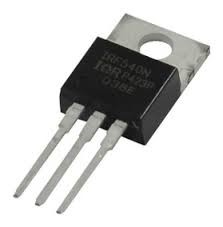
\includegraphics[width=2.06in,height=1.74in]{./media/image2.jpg}
	\end{Center}
\end{figure}


%%%%%%%%%%%%%%%%%%%% Figure/Image No: 2 Ends here %%%%%%%%%%%%%%%%%%%%

\setlength{\parskip}{15.96pt}
\par


\vspace{\baselineskip}

\vspace{\baselineskip}

\vspace{\baselineskip}

\vspace{\baselineskip}

\vspace{\baselineskip}
\setlength{\parskip}{8.16pt}
\section{Características técnicas de elementos activa dores}
\setlength{\parskip}{8.04pt}
La lista de \textit{¸características ideales de trabajo de los transistores$"$  }describe elementos activadores en condiciones ideales, pero ese es el problema que la mayoría de estos dispositivos semiconductores no trabaja en esas condiciones por lo cual, cada fabricante diseña una hoja de datos técnicos en los cuales da a conocer la forma de trabajar de cada dispositivo, la hoja está determinada como \textit{Datasheets }la cual es propia del dispositivo, fabricante y encapsulado.\par

\setlength{\parskip}{11.52pt}
Lo importante en esta sección será el cálculo de esas condiciones en las que debe trabajar un transistor para funcionar con un circuito, el cual está dado por las siguientes características:\par

\setlength{\parskip}{8.52pt}
\begin{adjustwidth}{0.25in}{0.0in}
Capacidades de voltaje\par

\end{adjustwidth}

\begin{adjustwidth}{0.25in}{0.0in}
Capacidades de corriente\par

\end{adjustwidth}

\setlength{\parskip}{33.96pt}
\begin{adjustwidth}{0.25in}{0.0in}
Velocidad o frecuencia de interrupción\par

\end{adjustwidth}

\setlength{\parskip}{0.0pt}
De manera más visual podemos observar en la figura 2 como es que diferentes tipos de transistores trabajan con sus capacidades máximas en cuanto voltajes y corrientes:\par



%%%%%%%%%%%%%%%%%%%% Figure/Image No: 3 starts here %%%%%%%%%%%%%%%%%%%%

\begin{figure}[H]
	\begin{Center}
		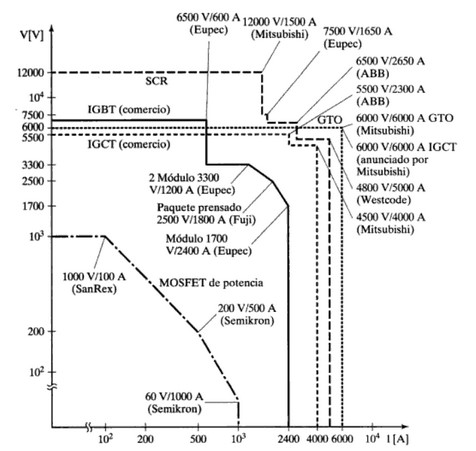
\includegraphics[width=4.21in,height=4.34in]{./media/image3.jpg}
	\end{Center}
\end{figure}


%%%%%%%%%%%%%%%%%%%% Figure/Image No: 3 Ends here %%%%%%%%%%%%%%%%%%%%

\par


\vspace{\baselineskip}
\setlength{\parskip}{8.04pt}

\vspace{\baselineskip}
\section{Características de los dispositivos prácticos}
\setlength{\parskip}{4.2pt}
\begin{adjustwidth}{-0.01in}{-0.01in}
Estos tipos de transistores con conmutación trabajan con determinados tiempos, los cuales están definidos como los siguientes: un tiempo de demora tiempo de subida tiempo de almacenamiento tiempo de bajada\par

\end{adjustwidth}

\setlength{\parskip}{0.0pt}
De manera tal que cuando la corriente satura y comienza con el tiempo de subida, de manera contraria el voltaje comenzara con su tiempo de bajada, y cuando la corriente trabaje en el tiempo de bajada el voltaje iniciara la subida, el tiempo de cerrado de un dispositivo es la suma del tiempo de retardo y el tiempo de subida, algo así como lo muestran la imagen 3:\par



%%%%%%%%%%%%%%%%%%%% Figure/Image No: 4 starts here %%%%%%%%%%%%%%%%%%%%

\begin{figure}[H]
	\begin{Center}
		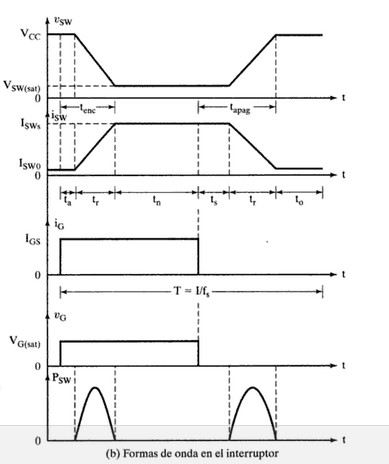
\includegraphics[width=3.24in,height=3.87in]{./media/image4.jpg}
	\end{Center}
\end{figure}


%%%%%%%%%%%%%%%%%%%% Figure/Image No: 4 Ends here %%%%%%%%%%%%%%%%%%%%

\setlength{\parskip}{15.96pt}
\par

\setlength{\parskip}{24.84pt}
Figura 3: diferentes ondas con las que trabaja un transistor de potencia\par

\setlength{\parskip}{7.92pt}
\begin{adjustwidth}{0.25in}{0.0in}
La pérdida promedio de potencia de potencia en la conducción \textit{P\textsubscript{e}nca }está determinada por:\par

\end{adjustwidth}



%%%%%%%%%%%%%%%%%%%% Figure/Image No: 5 starts here %%%%%%%%%%%%%%%%%%%%

\begin{figure}[H]
	\begin{Center}
		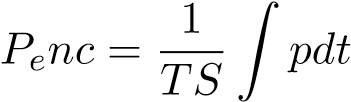
\includegraphics[width=1.17in,height=0.34in]{./media/image5.png}
	\end{Center}
\end{figure}


%%%%%%%%%%%%%%%%%%%% Figure/Image No: 5 Ends here %%%%%%%%%%%%%%%%%%%%

\setlength{\parskip}{4.32pt}
 \tabto{3.39in}  \tabto{6.69in} (1)\par

\setlength{\parskip}{0.0pt}
La pérdida de conmutación que resulta, Psi durante los periodos de cerrado ya abierto se determina con:\par


\vspace{\baselineskip}
\setlength{\parskip}{29.88pt}


%%%%%%%%%%%%%%%%%%%% Figure/Image No: 6 starts here %%%%%%%%%%%%%%%%%%%%

\begin{figure}[H]
	\begin{Center}
		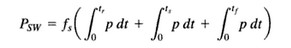
\includegraphics[width=1.62in,height=0.27in]{./media/image6.jpg}
	\end{Center}
\end{figure}


%%%%%%%%%%%%%%%%%%%% Figure/Image No: 6 Ends here %%%%%%%%%%%%%%%%%%%%

\par


\vspace{\baselineskip}

\vspace{\baselineskip}

\vspace{\baselineskip}
\setlength{\parskip}{12.84pt}
\begin{adjustwidth}{0.25in}{0.0in}
Las especificaciones que debe de mantener son las siguientes:\par

\end{adjustwidth}

\setlength{\parskip}{4.2pt}
\begin{adjustwidth}{0.39in}{-0.01in}
 capacidades de voltaje: voltajes pico repetitivos directo e inverso y caída de voltaje den directo en el estado cerrado. capacidades corrientes: corrientes y promedio, raíces cuadráticas media.\par

\end{adjustwidth}

\setlength{\parskip}{4.08pt}
\begin{adjustwidth}{0.25in}{0.0in}
velocidad o frecuencia de interrupción, cambio de un estado totalmente conductor hasta un estado totalmente no conductor, son parámetros muy importantes el periodo y la frecuencia de interrupción, que están dadas por:\par

\end{adjustwidth}


\vspace{\baselineskip}
\setlength{\parskip}{17.28pt}


%%%%%%%%%%%%%%%%%%%% Figure/Image No: 7 starts here %%%%%%%%%%%%%%%%%%%%

\begin{figure}[H]
	\begin{Center}
		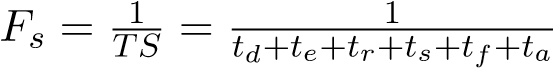
\includegraphics[width=2.24in,height=0.36in]{./media/image7.png}
	\end{Center}
\end{figure}


%%%%%%%%%%%%%%%%%%%% Figure/Image No: 7 Ends here %%%%%%%%%%%%%%%%%%%%

\par


\vspace{\baselineskip}
\setlength{\parskip}{8.04pt}

\printbibliography
\end{document}